\documentclass[a4paper,12pt]{article}
\author{Adam Ilyas}
\title{
CS-E4850 Computer Vision, \\
Answers to Exercise Round 2
}

\pagestyle{empty}

% \usepackage{t1enc}
\usepackage{a4wide}
\usepackage{amsfonts}
\usepackage{verbatim}
\usepackage{amsmath}
\usepackage{amssymb}
\usepackage{graphicx}
\usepackage[english]{babel}

\begin{document}
\vspace{8pt}

\maketitle

\section{Pinhole Camera}
The perspective projection equations for a pinhole camera are
\begin{equation}
\begin{split}
x_p = f\frac{x_c}{z_c}, \quad y_p = f\frac{y_c}{z_c}, 
\end{split}
\end{equation}
where $\mathbf{x}_p = [x_p,y_p]^\intercal$ are the projected coordinates on the image plane, $\mathbf{x}_c = [x_c,y_c,z_c]^\intercal$ is the imaged point in the camera coordinate frame and $f$ is the focal length. Give a geometric justification for the perspective projection equations.
\begin{figure}[!ht]
	\begin{center}
    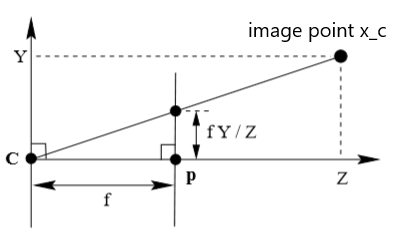
\includegraphics[scale=0.8]{pic1.png}
    \caption{Similar triangles}
	\end{center}
\end{figure}\\
Since $\triangle CZ\mathbf{x}_c$ and $\triangle Cp\mathbf{x}_p$ are similar triangles: $$\frac{y_c}{z_c} = \frac{y_p}{f}, \quad y_p = f\frac{y_c}{z_c}$$Since the image plane is parallel to the xy-plane (principal plane which is a plane that goes through the camera centre), similar triangles can be applied to the x-coordinates $$\frac{x_c}{z_c} = \frac{x_p}{f}, \quad x_p = f\frac{x_c}{z_c}$$

\section{Pixel Coordinate Frame} 
The image coordinates $x_p$ and $y_p$ given by the perspective projection equations (1) above are not in pixel units. The $x_p$ and $y_p$ coordinates have the same unit as distance $f$ (typically millimetres) and the origin of the coordinate frame is the principal point (the point where the optical axis pierces the image plane). Now, give a formula which transforms the point $x_p$ to its pixel coordinates $\mathbf{p} = [u,v]^\intercal$ when the number of pixels per unit distance in $u$ and $v$ directions are $m_u$ and $m_v$, respectively, the pixel coordinates of the principal point are $(u_0,v_0)$ and \\ a) u and v axis are parallel to x and y axis respectively.
\\ b) u axis is parallel to x axis and the angle between u and v axis is $\theta$. \\\\
\textbf{Solution}\\
a) if u and v axis are parallel to x and y axis \\
We want to transform image coordinate to $(x_p, y_p)^\intercal \mapsto (u,v)^\intercal$ pixel coordinate by doing so
\[
\begin{pmatrix}
    m_x & 0 & 0 \\
    0 & m_y & 0 \\
    0 & 0 & 1
\end{pmatrix}
\begin{pmatrix}
    f\frac{x_c}{z_c} + p_x \\
    f\frac{y_c}{z_c} + p_y\\
    1
\end{pmatrix} = 
\begin{pmatrix}
    m_xf\frac{x_c}{z_c} + m_xp_x \\
    m_yf\frac{y_c}{z_c} + m_yp_y\\
    1
\end{pmatrix} =
\begin{pmatrix}
    m_xx_p + u_0 \\
    m_yy_p + v_0\\
    1
\end{pmatrix} 
\]
We represent the image coordinates of the principal point be $[p_x,p_y]^\intercal$. The formula to transform the point $x_p$ to pixel coordinates is:
$$u = m_ux_p + u_0, \quad v = m_vy_p + v_0$$\\
b) u axis is parallel to x axis and the angle between u and v axis is $\theta$
\begin{center}
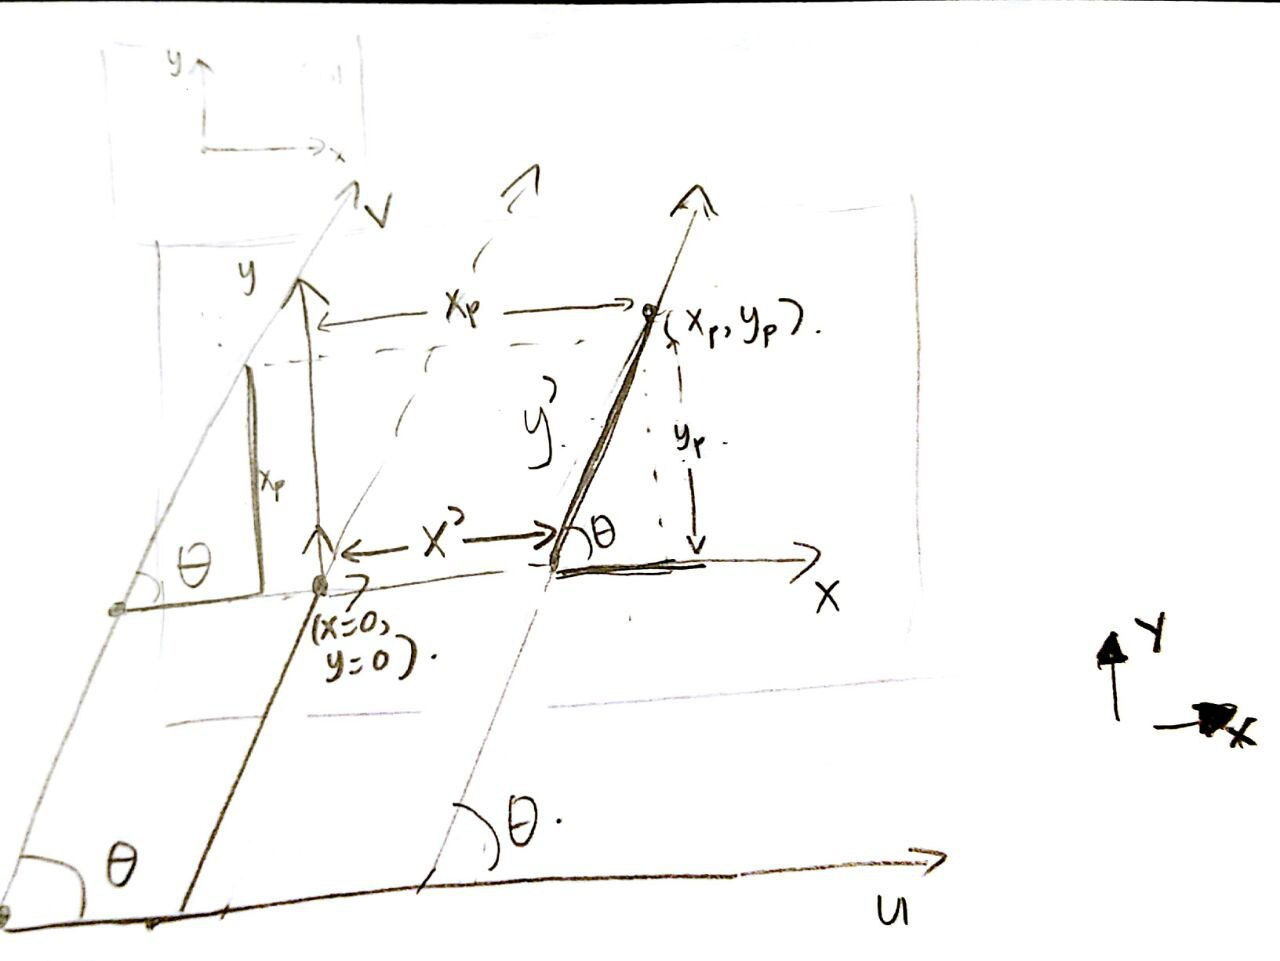
\includegraphics[scale=0.25]{cv_2.jpg}
\end{center}
From the diagram above, in particular, we are interested in $x^\prime$ and $y^\prime$:
$$\frac{y_p}{y^\prime} = sin(\theta), \quad y^\prime= \frac{1}{sin(\theta)}y_p$$
$$\frac{y_p}{x_p - x^\prime} = \tan \theta, \quad x^\prime = x_p - \frac{1}{tan(\theta)}y_p$$
Once we considered the rotation of the new coordinates, we can modify the scale and shift of the image coordinate to the new pixel coordinates
\begin{equation}
\begin{split}
u = m_ux^\prime + u_0, \quad \quad \quad& \quad v = m_v y^\prime + v_0\\
u = m_u x_p - \frac{m_u}{tan(\theta)}y_p + u_0, & \quad v = m_v \frac{1}{sin(\theta)}y_p + v_0
\end{split}
\end{equation}

\section{Intrinsic camera calibration matrix}
Use homogeneous coordinates to represent case (2.b) above with a matrix $\mathbf{K}_{3\times 3}$, also known as the camera's intrinsic calibration matrix, so that $\mathbf{\tilde{p} = \mathbf{Kx}_c}$. Where $\tilde{\mathbf{p}}$ is $\mathbf{p}$ in homogeneous coordinates.\\\\
\textbf{Solution}\\
We want to find $\mathbf{K}_{3\times 3}$ such that:
$$
\mathbf{K}_{3\times 3}
\begin{pmatrix}
x_c \\
y_c \\
z_c
\end{pmatrix} = 
\begin{pmatrix}
u\\
v\\
1
\end{pmatrix}
$$
From section 2.B:
\begin{equation}
\begin{split}
\begin{pmatrix}
u\\v\\1
\end{pmatrix} & = 
\begin{pmatrix}
    m_u & -\frac{m_u}{\tan \theta} & u_0\\
    0 & m_v (1 /\sin \theta) & v_0\\
    0 & 0 & 1
\end{pmatrix} 
\begin{pmatrix}
x_p\\y_p\\1
\end{pmatrix} \\
& = 
\begin{pmatrix}
    m_u & -\frac{m_u}{\tan \theta} & u_0\\
    0 & m_v (1 /\sin \theta) & v_0\\
    0 & 0 & 1
\end{pmatrix} 
\begin{pmatrix}
fx_c\\fy_c\\fz_c
\end{pmatrix}
\end{split}
\end{equation}

\section{ Camera projection matrix}
Imaged points are often expressed in an arbitrary frame of reference called the world coordinate frame. The mapping from the world frame to the camera coordinate frame is a rigid transformation consisting of a 3D rotation R and translation t: $$x_c = \mathbf{R}x_w + \mathbf{t}$$ Use homogeneous coordinates and the result of the exercise 3 above, to write down the $3 \times 4$ camera projection matrix P that projects a point form world coordinates $x_w$ to pixel coordinates. That is, represent P as a function of the internal camera parameters K and the external camera parameters R,t.\\\\
The world $\mapsto$ pixel camera matrix :
$$\begin{pmatrix}
u\\v\\1
\end{pmatrix} = \mathbf{K}\tilde{x}_c = \mathbf{K}(\mathbf{R}\tilde{x}_w + t) = \mathbf{K}[\mathbf{R} \quad t]
\begin{pmatrix}
\tilde{x}_w\\1
\end{pmatrix} = \mathbf{P} 
\begin{pmatrix}
\tilde{x}_w\\1
\end{pmatrix}
$$ 
\end{document}
